\documentclass[11pt,a4paper]{article}
\usepackage[margin=1in]{geometry}
\usepackage{amsmath,amssymb,amsthm}
\usepackage{booktabs}
\usepackage{array}
\usepackage{fontspec}
\setmainfont{lmroman10-regular.otf}[
  BoldFont=lmroman10-bold.otf,
  ItalicFont=lmroman10-italic.otf,
  BoldItalicFont=lmroman10-bolditalic.otf,
]
\setmonofont{Menlo}[Scale=0.86, Ligatures=NoCommon]
\usepackage{microtype}
\usepackage{xcolor}
\definecolor{seclink}{HTML}{1F4E8C}
\usepackage[colorlinks=true,linkcolor=seclink,citecolor=seclink,urlcolor=blue]{hyperref}
\usepackage{parskip}
\usepackage{fancyvrb}
\usepackage{tikz}
\usepackage[most]{tcolorbox}

\definecolor{yellowbg}{HTML}{FBF3D5}
\definecolor{pinkbg}{HTML}{FADDE1}
\definecolor{bluebg}{HTML}{E8EEF7}

\tcbset{plainbg/.style={boxrule=0pt, sharp corners, colframe=white,
  left=4mm, right=4mm, top=3mm, bottom=3mm, before skip=3mm, after skip=3mm,
  before upper={\setlength{\parskip}{0.6\baselineskip}}}}
\newtcolorbox{sectionbox}{plainbg, colback=yellowbg}
\newtcolorbox{alarmbox}{plainbg, colback=pinkbg}
\newtcolorbox{notebox}{plainbg, colback=bluebg}

\DefineVerbatimEnvironment{term}{Verbatim}{fontsize=\footnotesize, xleftmargin=0mm}

\newtheorem*{claim}{Claim}
\newtheorem*{obs}{Observation}

\title{\vspace{-2em}Coherence}
\author{\normalsize When A and B federate, and B and C federate,\\[0.2em]
\normalsize and A and C do not}
\date{\normalsize Claude, 7 September 2026}

\begin{document}
\maketitle
\vspace{-1em}

\begin{sectionbox}
Robin put the following picture. Two polities A and B can federate well, with
good trade and a working political alliance. Two polities B and C can federate
well on the same terms. And A and C can fail to federate.

That picture is not the obstruction the M\"obius programs compute. It is the one
degree above it, and the two failures are qualitatively different rather than
two sizes of the same thing. In the M\"obius ring every pairwise relation works
and there is still no global answer. In this picture the pairwise relations work
and do not compose.

The distinction matters because the second failure is worse. It says there is no
federation to have an answer about.

It also turns out that the picture as stated does not settle which failure it
is. Whether A and C failing is a coherence failure or more monodromy depends on
a fact the labels do not record, namely whether anything at all falls under A,
B and C at once.

And the two degrees are not independent. Admitting one triple overlap either
removes a monodromy class or creates a coherence class, never both and never
neither, so the total obstruction is conserved. The one manoeuvre practitioners
have against a coherence failure does not remove it. It moves it down a degree,
where every pairwise check will pass and the obstruction is still there.

It ends by noticing who profits, which is not either of the parties that
federated.
\end{sectionbox}

\section{The two failures}

Write $g_{AB}$ for the transition function on the overlap of A and B. It is the
translation between A's frame and B's, and in \texttt{mobius.pdf} it lives in
the backward map of a container morphism and nowhere else.

\medskip
\textbf{Degree one, monodromy.} Every $g_{ij}$ is well formed, so the transition
data does define a glued object. The product of the transitions around a cycle
is not the identity, so that object has no global section. This is what
\texttt{./mobius class} reports and what \texttt{./mobius glue -\/-detect}
accumulates in the ring.

\medskip
\textbf{Degree two, coherence.} On the region where three parties all have
authority, the transitions must compose:
\[
  g_{AB} \cdot g_{BC} = g_{AC}
  \qquad\text{on}\qquad
  U_A \cap U_B \cap U_C .
\]
Robin's picture is exactly this equation failing. Going from A to C through B
and going from A to C directly disagree.

\begin{alarmbox}
\textbf{They are not degrees of one thing.}

Monodromy is a well-defined federation with no possible common policy. The
sheaf exists. It has no global section. There is an object, and it has no
answer.

A coherence failure is not that. The transitions do not compose, so they do not
define a sheaf at all. One cannot ask whether a global section exists, because
the thing that would have sections was never constructed. There are three
bilateral relationships that contradict each other on the region where all
three apply, and no federation.
\end{alarmbox}

Note what the equation needs in order to fail. It needs $U_A \cap U_B \cap U_C$
to be non-empty. If no matter falls under all three authorities at once then
the equation has no domain, it holds vacuously, and coherence cannot fail. That
is the situation the existing program is in, and \texttt{./mobius nerve} says so
in as many words.

\begin{term}
  THE NERVE

    arcs                    3
    dim C0, C1, C2          3, 3, 0
    Z1 = C1                 rank 3   (d1 lands in 0)
    B1 = im d0              rank 2   (ker d0 = the constants)
    H1 = Z1/B1              Z/2

    The triple overlap is empty, so the cocycle condition is VACUOUS.
    This demonstrates monodromy. It does not exercise coherence.
\end{term}

\section{Which failure it is, and why the labels do not say}

Put four polities in a ring. A federates with B, B with C, C with D, and D with
A. And A and C fail to federate. That statement is not yet enough to locate the
failure, and the arithmetic of the three readings differs.

\begin{term}
=== four patches: A-B, B-C, C-D, D-A all federate, and A-C does not ===
  no A-C relation at all                       E=4 F=0  chi=  0   H1=1  H2=0   classes=2
  A-C exists, triple overlaps ALL empty        E=5 F=0  chi= -1   H1=2  H2=0   classes=4
  A-C exists, triple ABC nonempty              E=5 F=1  chi=  0   H1=1  H2=0   classes=2
  A-C exists, triples ABC and ACD              E=5 F=2  chi=  1   H1=0  H2=0   classes=1
\end{term}

\textbf{If A and C have no overlap}, nothing is failing. The relation is absent
rather than broken. That is the first line, a four-patch ring with two classes,
and it is the M\"obius demonstration with one more node.

\textbf{If A and C overlap and every triple overlap is empty}, the second line,
there is no cocycle condition anywhere, so the failure cannot be a coherence
failure. What it can be is non-trivial holonomy around the triangle A, B, C.
That is still monodromy, in degree one. Note the class count. Adding the A--C
relation gives the nerve a second independent loop, the triangles ABC and ACD,
so there are \emph{four} classes rather than two.

\textbf{If A, B and C share a region}, the third line, then and only then does
$g_{AB} \cdot g_{BC} = g_{AC}$ have a domain, and A and C failing can mean the
equation failing. That is the coherence reading, and it is the design of \S4.

\begin{sectionbox}
\textbf{The distinguishing question is not about A and C.} It is whether any
matter falls under A, B and C simultaneously. Three working bilateral
relationships and one broken one is compatible with there being no coherence
question at all.

Put politically: two parties can be in conflict over a third party's conduct
without there being anything the three of them jointly govern, and in that case
the failure is a loop rather than a contradiction.
\end{sectionbox}

\section{Three patches cannot show both failures}

The empty triple overlap in that cover has been described in the repository as
a limitation. It is not a choice. It is forced, and the reason is worth having
in front of us before designing anything.

By the nerve lemma, a cover all of whose non-empty intersections are
contractible has a nerve homotopy equivalent to the space. So the nerve of a
good cover of the circle must be homotopy equivalent to the circle. The
cohomology of these nerves was computed over $\mathbb{F}_2$ by building the
boundary maps and taking ranks.

\begin{term}
=== nerves of covers, cohomology over F2 ===
  3 arcs, triple overlap empty       V=  3 E=  3 F=  0  chi=  0   H0=1 H1=1 H2=0   triples: NONE
  3 arcs, triple overlap NONempty    V=  3 E=  3 F=  1  chi=  1   H0=1 H1=0 H2=0   triples: yes
  4 arcs, all triples empty          V=  4 E=  4 F=  0  chi=  0   H0=1 H1=1 H2=0   triples: NONE
  4 arcs, ONE triple nonempty        V=  4 E=  5 F=  1  chi=  0   H0=1 H1=1 H2=0   triples: yes
\end{term}

Read the first two lines together.

\begin{sectionbox}
\textbf{With three patches you must choose which failure you are modelling.}
Leave the triple overlap empty and the nerve is a hollow triangle, so
$H^1 = \mathbb{Z}/2$ and there is monodromy to exhibit, but the cocycle
condition has no domain. Fill the triple overlap and the nerve becomes a solid
triangle, which is contractible, so $H^1 = 0$ and the monodromy is destroyed.

The three-arc cover in the program is therefore not a lazy cover. It is the
only three-patch cover of the circle that has anything to show, and the price
of having it is that coherence is unreachable.
\end{sectionbox}

\section{Four patches, and having both}

The fourth line of that output is the design. Four patches, five overlaps, one
genuine triple overlap, and $H^1$ still $\mathbb{Z}/2$. The Euler
characteristic is zero and the nerve is homotopy equivalent to the circle, so
this is a good cover of $S^1$ and the two-class arithmetic survives intact.

It is realisable, and here it is. Give the circle degree coordinates and take
four arcs, written as intervals running anticlockwise.
\[
  U_A = (70, 220), \quad
  U_B = (75, 105), \quad
  U_C = (320, 110), \quad
  U_D = (200, 340).
\]
Three of them, $U_A$, $U_B$ and $U_C$, contain the point $p$ at $90$ degrees.
The fourth covers the far side and does not reach $p$.

\begin{center}
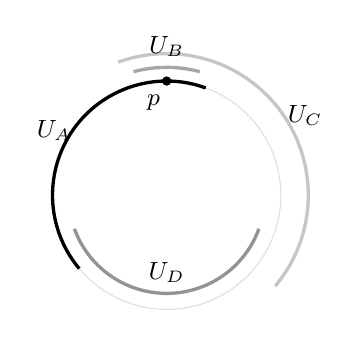
\begin{tikzpicture}[scale=1.45, every node/.style={font=\small}]
  \draw[gray!25] (0,0) circle (1);
  \draw[very thick]              (70:1.00)  arc (70:220:1.00);
  \draw[very thick, gray!70]     (75:1.12)  arc (75:105:1.12);
  \draw[very thick, gray!45]     (-40:1.24) arc (-40:110:1.24);
  \draw[very thick, gray!85]     (200:0.86) arc (200:340:0.86);
  \node at (150:1.14) {$U_A$};
  \node at (90:1.30)  {$U_B$};
  \node at (30:1.40)  {$U_C$};
  \node at (270:0.68) {$U_D$};
  \node[circle, fill=black, inner sep=1.2pt] at (90:1) {};
  \node at (98:0.82) {$p$};
\end{tikzpicture}
\hspace{1.4cm}
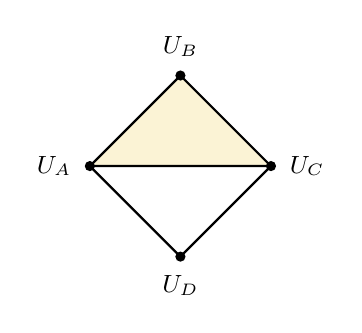
\begin{tikzpicture}[scale=1.15, every node/.style={font=\small}]
  \fill[yellowbg] (0,0) -- (1,1) -- (2,0) -- cycle;
  \draw[thick] (0,0) -- (1,1) -- (2,0) -- (0,0);
  \draw[thick] (0,0) -- (1,-1) -- (2,0);
  \node[circle, fill=black, inner sep=1.3pt] at (0,0)  {};
  \node[circle, fill=black, inner sep=1.3pt] at (1,1)  {};
  \node[circle, fill=black, inner sep=1.3pt] at (2,0)  {};
  \node[circle, fill=black, inner sep=1.3pt] at (1,-1) {};
  \node[left]  at (-0.1,0)   {$U_A$};
  \node[above] at (1,1.1)    {$U_B$};
  \node[right] at (2.1,0)    {$U_C$};
  \node[below] at (1,-1.1)   {$U_D$};
\end{tikzpicture}
\end{center}

\vspace{-0.4em}
\noindent
On the right is the nerve. One filled triangle, one hollow one, sharing the
edge from $U_A$ to $U_C$. The hollow half is the hole that carries $H^1$, and
the filled half is the triple overlap.

The cover was checked rather than eyeballed. The circle was sampled finely, the
intersections computed, and their components counted.

\begin{term}
covers the circle: True

pairs:
  AB: nonempty  components 1        triples:
  AC: nonempty  components 1          ABC: nonempty  components 1
  AD: nonempty  components 1          ABD: EMPTY     components 0
  BC: nonempty  components 1          ACD: EMPTY     components 0
  BD: EMPTY     components 0          BCD: EMPTY     components 0
  CD: nonempty  components 1        ABCD: EMPTY

nerve: V=4  E=5 ['AB', 'AC', 'AD', 'BC', 'CD']  F=1 ['ABC']   chi = 0
\end{term}

Every non-empty intersection is a single arc, so the cover is good and the nerve
lemma applies. There is exactly one triple overlap. The Euler characteristic is
zero, matching the fourth line of \S2, so the first cohomology is still
$\mathbb{Z}/2$ and the two classes survive.

Note which intersections have to be empty and why. The arc $U_B$ must not reach
$U_D$, or the nerve acquires a second face and the hole closes. And $U_A \cap
U_C$ must stay on the near side of the circle, away from $U_D$, or the triple
$ACD$ becomes non-empty and does the same thing. The design is tighter than it
looks.


So a four-arc ring can run Robin's picture as a live demonstration. Set
$g_{AB}$ and $g_{BC}$ to whatever is wanted, set $g_{AC}$ to something that is
not their product, and the program has A and B federating, B and C federating,
and A and C failing, on a cover where that statement is not vacuous.

\section{The obstruction budget}

The four lines in \S2 do something more than distinguish three readings. Read
down the $H^1$ column as triple overlaps are admitted. Two classes, then four,
then two, then one. Each triple overlap admitted drops $H^1$ by exactly one.

That is a theorem rather than a pattern, and the proof is one line. Adding a
single 2-simplex raises the Euler characteristic by one. Since
$\chi = H^0 - H^1 + H^2$, it must either drop $H^1$ by one or raise $H^2$ by
one. The other branch is not hypothetical. Closing the fourth face of a
tetrahedron raises $H^2$ from zero to one and leaves $H^1$ alone.

\begin{term}
=== the other branch: a face can raise H2 instead of dropping H1 ===
  tetrahedron, 3 of its 4 faces                E=6 F=3  chi=  1   H1=0  H2=0   classes=1
  tetrahedron, all 4 faces                     E=6 F=4  chi=  2   H1=0  H2=1   classes=1
\end{term}

\begin{sectionbox}
\textbf{The obstruction is conserved.} A triple overlap does not add an
obstruction and does not remove one. It converts a monodromy class into a
coherence condition. Emptying a triple overlap runs the conversion backwards.

So the two degrees are not two independent problems to be solved separately.
They are one quantity, and admitting or refusing a triple overlap chooses which
degree it is expressed in.
\end{sectionbox}

\section{Where the picture is the shape of things}

The canonical instance has Australia standing in it.

Australia and China have the largest trading relationship. Australia and the
United States have the security alliance. The United States and China are in
strategic competition. Two edges work and the third does not, and the failure is
not a lack of Australian goodwill or competence. On the region where both
relationships apply, which is critical minerals, semiconductors, network
equipment, port leases, research collaboration and strategic exports, the two
transitions disagree. No single Australian policy restricts correctly to both.

Four more of the same shape.

\begin{center}
\begin{tabular}{@{}>{\raggedright\arraybackslash}p{4.0cm}>{\raggedright\arraybackslash}p{9.3cm}@{}}
\toprule
\textbf{triple} & \textbf{how it failed} \\
\midrule
Australia, UK, US
  & Forming this triple in 2021 broke the working Australia--France
    relationship. The cancelled submarine contract was the price of composing
    it. \\
Turkey, NATO, Russia
  & A NATO member buying Russian air defence. Expulsion from the F-35
    programme was the concrete cost of the transitions not composing. \\
Australia, UK, EU
  & The Australia--UK agreement entered into force in 2023 and a UK--EU
    agreement is in place, while Australia--EU negotiations collapsed twice
    over agricultural access and critical minerals. \\
Scotland, UK, EU
  & Scotland is in a union with the UK, voted 62\% to remain in the EU, and the
    UK left. Scotland's local data cannot restrict consistently to both. \\
\bottomrule
\end{tabular}
\end{center}

The last row is where this note started, and it is worth being exact about it.
Robin's original observation was that Australia and Scotland share language,
culture and diaspora, so cooperation between them is straightforward. That is
right, and in container terms it says the transition function on that overlap is
near the identity. What follows is that the Australia--Scotland edge is the easy
one, and the easy edge is not where anything is decided. The loop runs through
Westminster, and the class sits on the Scotland--UK edge.

\section{What compartmentalisation actually does}

Practitioners have a standard response, and it has a precise description.

They shrink the overlap. Trade is separated from security. A matter is declared
commercial rather than strategic. Sensitive sectors get carve-outs. Stated
mathematically, all of that is \textbf{refining the cover until the triple overlap
is empty}. The cocycle condition becomes vacuous and the coherence failure can
no longer be expressed, because the equation has no domain on which to hold.

An earlier draft of this note said that the failure is thereby dissolved. That
is wrong, and the budget of \S5 is what makes it wrong. Emptying a triple
overlap raises $H^1$ by one. The obstruction is not destroyed. It reappears one
degree down as monodromy.

\begin{alarmbox}
\textbf{And monodromy is the harder of the two to see.} A coherence failure
announces itself. Three parties look at one region and two of the routes across
it disagree, and any of them can point at the contradiction. Monodromy passes
every pairwise check. Every bilateral relationship is in good order, every
overlap is consistent, and there is still no global policy, and no audit of any
pair will find it.

So carving up the overlap does not remove the obstruction. It makes the
obstruction invisible to exactly the kind of inspection that institutions
perform, which is bilateral.
\end{alarmbox}

The political reading follows without extra machinery. Separate trade from
security, and each basket becomes internally consistent, and every bilateral
relationship works, and there is still no coherent strategy. That is not a
failure of the compartmentalisation. It is what compartmentalisation does.

The purest example is the Northern Ireland Protocol. Northern Ireland lies in
the overlap of the UK internal market and the EU single market, and the two
transitions disagree there. The border in the Irish Sea was a refinement of the
cover. The Windsor Framework's green and red lanes are a finer refinement,
carving the overlap into pieces on which only one transition applies. Years of
negotiation, and the substance of it is cover refinement rather than agreement.

\section{And the condition under which it is unavailable}

The conversion is not always available either, and whether it is available is a
fact about the space rather than about the negotiators.

A space of covering dimension one admits covers with empty triple overlaps.
Three arcs on a circle achieve exactly that. A space of dimension two does not.
Any good cover of a surface has non-empty triple overlaps, and no refinement
removes them.

\begin{sectionbox}
\textbf{Compartmentalisation works exactly when the polity is one-dimensional.}
If the jurisdictions form a chain or a ring, each meeting only its neighbours,
one can always carve until the triple overlaps vanish, and what survives is
monodromy alone.

If there are matters that fall under three authorities at once, irreducibly,
then the polity has dimension two or more, no carve-out empties the triple, and
the coherence failure is permanent. On that reading Northern Ireland is
intractable because it is a two-dimensional problem being handed
one-dimensional instruments.
\end{sectionbox}

That also justifies the existing program in a way the repository has not
claimed. The M\"obius ring models a federation that has already
compartmentalised successfully, and the obstruction it finds is what every
carve-out has left behind. A coherence failure can be pushed down a degree. The
loop it becomes cannot be pushed anywhere.

\section{What the class would be, and what it would not be}

Two honest limits on building this, both of which bear on how much it would
show.

\medskip
\textbf{The classifying object is a gerbe, not a sign.} With non-abelian
coefficients the second cohomology needs a band, and what it classifies is
gerbes rather than bundles. That is real machinery in the sense of Giraud, and
it is not one more sign in an array. Degree one was small because
$\mathbb{Z}/2$ is small. Degree two will not be.

\medskip
\textbf{The circle has no room for the class.} Look again at the fourth line of
the computation in \S2. The four-arc nerve has a genuine triple overlap and
$H^2 = 0$. So a four-arc cover of the circle lets one violate the cocycle
condition and watch the violation, and it supplies nothing to classify the
violation with. For a non-zero class in degree two the base must be
two-dimensional.

\begin{term}
  the torus (4x4 triangulated)       V= 16 E= 48 F= 32  chi=  0   H0=1 H1=2 H2=1   triples: yes

  genus-2 surface, CW: 1 vertex, 4 edges, 1 face on [a,b][c,d]
  the attaching word abelianises to zero, so both boundary maps vanish:
  H0=1 H1=4 H2=1   chi = 1-4+1 = -2 = 2-2g for g=2
\end{term}

The genus-two surface is the natural base and it arrives with three things at
once. The fundamental group becomes non-abelian, so the two directions round a
loop stop agreeing. The first cohomology has rank four over $\mathbb{F}_2$,
giving sixteen line bundles rather than two. And the second cohomology is
non-zero, so there is somewhere for a coherence class to live and a cup product
pairing the first cohomology into it.

\section{What is demonstrated and what is modelling}

\begin{alarmbox}
\textbf{Demonstrated here.} The cohomology over $\mathbb{F}_2$ of every nerve
in \S2, \S3, \S5 and \S8, computed from boundary maps by rank. In particular
that filling the triple overlap of a three-patch cover sends $H^1$ to zero,
that the four-arc cover of \S4 is a good cover with exactly one triple overlap
and $H^1 = \mathbb{Z}/2$, verified by sampling the circle, and that each triple
overlap admitted moves one obstruction from degree one to degree two.

\textbf{Corrected here.} An earlier draft said compartmentalisation dissolves a
coherence failure. It converts it into monodromy. The scripts are
\texttt{nerve-cohomology.py}, \texttt{four-arc-cover.py} and
\texttt{obstruction-budget.py}, beside this document.

\textbf{Solid, and none of it mine.} The nerve lemma. The cocycle condition and
its role in descent. The relation between covering dimension and the order of
overlaps a cover can be refined to avoid. Giraud on non-abelian second
cohomology and gerbes.

\textbf{Reporting.} The events in \S4 and \S5 are public and my
characterisations of them are ordinary ones. Figures and dates in this note
should be checked before quotation, since my information has a cutoff.

\textbf{Modelling, and contestable at exactly this step.} That jurisdictions
form a space at all, so that words like cover, overlap and dimension apply to
them. Everything in \S6 depends on that and on nothing else. If jurisdictions
are merely a set with pairwise and triple-wise intersections, and not a space
with a dimension, then the claim about when compartmentalisation is available
has no content. That is the question to put to a referee, and it is the same
question \texttt{sheaf-federation.pdf} already flags about its own site.
\end{alarmbox}

\section{What to build}

The four-arc ring, to the design in \S4. Three arcs sharing a point and a
fourth covering the far side, five overlaps, one triple. Then set $g_{AC}$ to
something other than $g_{AB} \cdot g_{BC}$ and the program exhibits Robin's
picture rather than disclaiming it.

The budget of \S5 makes the choice of how many triples to admit an explicit
design decision rather than an accident, and there are three defensible answers.

\begin{center}
\begin{tabular}{@{}>{\raggedright\arraybackslash}p{3.0cm}cc>{\raggedright\arraybackslash}p{6.4cm}@{}}
\toprule
\textbf{triples admitted} & \textbf{classes} & \textbf{conditions} & \textbf{what it demonstrates} \\
\midrule
none & 4 & 0 & richer monodromy, and no coherence \\
ABC & 2 & 1 & the picture, with the existing two-class story intact \\
ABC and ACD & 1 & 2 & pure coherence, monodromy fully spent \\
\bottomrule
\end{tabular}
\end{center}

The middle row is the one to build. It keeps the two classes the whole
repository is arranged around and makes the coherence question expressible at
the same time. The top row is a legitimate alternative and gives
\texttt{./mobius class} four answers instead of two.

That is worth doing on its own terms, because it converts the repository's
standing caveat into a demonstration. It will not produce a class, and the
output should say so in the same breath as it reports the violation, in the way
that \texttt{./mobius cover 2} reports its own $+1$ as $p^*\alpha = 0$ rather
than as a result.

The class needs a surface. That is the larger job and it is research rather
than implementation.

\section{A closing note, which is cynical}
\enlargethispage{2\baselineskip}

Notice who is comfortable in this picture.

B federates with A, and B federates with C, and the relation that fails is A
against C. B holds both, and B holds both precisely because nothing obliges B to
reconcile them. The cocycle condition constrains B's two treaties only on the
region where all three parties have authority. Off that region B is
unconstrained, and B's two relationships never have to be the same
relationship.

So a strategy falls out of the arithmetic. Maximise your pairwise overlaps and
refuse the triple ones. Be indispensable bilaterally and absent
multilaterally. Sell to both sides and sign nothing that requires the sides to
agree.

That is not a novel discovery, only an unusually exact statement of an old
practice. It is the entrep\^ot state, and the neutral banker, and the Swiss
cantons who supplied soldiers to every party in Europe and a guard to the Pope,
and the \emph{Garde \'Ecossaise} in France, and the Scots who fought for
Gustavus Adolphus while Scotland was at peace with his enemies.

\begin{sectionbox}
\emph{This is why it is always best to be a mercenary so that you can continue
to do trade with your enemies, between A and C.}
\end{sectionbox}

And there is a sting in it that the mathematics states rather than softens.
B's position is not merely comfortable. It is rent-bearing. What B's brokerage
is worth is exactly what A and C cannot do directly, so the value of being B is
the size of the failure between A and C.

Which means the mercenary's interest is in the cocycle condition continuing to
fail. A broker asked to help A and C reconcile is being asked to destroy his own
position, and will bring to that task precisely the enthusiasm one would expect.

The arithmetic does not say this is admirable. It says it is stable. Being a
node of a federation costs coherence, declining to be one costs nothing, and
neither degree rewards the parties who paid.

\end{document}
